%%%%%%%%%%%%%%%%%%%%%%%%%%%%%%%%%%%%%%%%%%%%%%%%%%%%%%%%%%%%%%%%%%%%%%%%%%%%%
%% MS Draft Journal of Ecology Special Issue, Dispersal - 
%% Pedro - 07 April 2016
%----------------------------------------------------------------------------
%%%%%%%%%%%%%%%%%%%%%%%%%%%%%%%%%%%%%%%%%%%%%%%%%%%%%%%%%%%%%%%%%%%%% Headers
\documentclass[a4paper, 12pt]{article}
\usepackage{graphicx}
\usepackage[utf8]{inputenc}
\usepackage[a4paper]{geometry}
\usepackage{hyperref}
\pagestyle{plain}
\usepackage{amsmath,amssymb}
\usepackage{geometry}
\usepackage{lscape}
\usepackage{setspace}
\usepackage{verbatim}
\usepackage{graphicx}
\usepackage{epstopdf}
\usepackage{booktabs}
\usepackage{natbib}
\usepackage{longtable}
\usepackage{rotating}                                                                                    
\newcommand{\tab}{\hspace{5mm}}
\usepackage{tabularx} 
\usepackage[margin=10pt,font=small,labelfont=bf]{caption}
\usepackage[left]{lineno}
\usepackage{caption}
\DeclareGraphicsRule{.tif}{png}{.png}{`convert #1 `basename #1 .tif`.png}
\usepackage{fancyhdr} % This should be set AFTER setting up the page geometry
\pagestyle{fancy}     % options: empty , plain , fancy
\renewcommand{\headrulewidth}{0pt} % customise the layout...
\lhead{{\tiny Jordano - What is long-distance dispersal?}}\chead{}\rhead{}
\lfoot{}\cfoot{\thepage}\rfoot{}
\usepackage{parskip}
%%%%%%%%%%%%%%%%%%%%%%%%%%%%%%%%%%%%%%%%%%%%%%%%%%%%%%%%%%%%%%%%%% Title page
\begin{document}


\title{Manuscript Draft\\
\vspace{2cm}
What is long-distance dispersal? And a taxonomy of dispersal events}

\author{Pedro Jordano$^{\dag}$}

\date{Sevilla, \today}
\maketitle


\begin{spacing}{1.0}
$^{\dag}$ {\small Integrative Ecology Group, Estaci\'on Biol\'ogica de 
Do\~nana, CSIC, Avda. Americo Vespucio, s/n, Isla de La Cartuja
E-41092 Sevilla, Spain.}\\


{\small \textit{Corresponding author:} Pedro Jordano. Integrative Ecology Group, Estaci\'on Biol\'ogica de Do\~nana, CSIC, Avda. americo Vespucio, s/n, E-41092 Sevilla, Spain. Email address: jordano@ebd.csic.es}\\

\textbf{Key words}: ***\\

{\small \textbf{Manuscript information: }** Words; ** Chars; ** Pages, * Figures; * Tables.}
\end{spacing}

\maketitle
\newpage

%%%%%%%%%%%%%%%%%%%%%%%%%%%%%%%%%%%%%%%%%%%%%%%%%%%%%%%%%%%%%%%%%%%% Abstract
\section*{Abstract}
\begin{linenumbers}

Dispersal is a key individual-based process influencing many life-history attributes, scaling up to population-level properties (e.g., metapopulation connectivity). A persistent challenge in dispersal ecology has been the robust characterization of dispersal functions (kernels), a fundamental tool to predict how dispersal processes respond under global change scenarios. Especially the rightmost tail of these functions, i.e. the long-distance dispersal (LDD) events, are difficult to characterize empirically and to model in realistic ways. But, when is it a LDD event? In the specific case of plants, dispersal has three basic components: 1) a distinct (sessile) source, the maternal plant producing the fruits or the paternal tree acting as a source of pollen; 2) a distance component between source and target locations; and 3) a vector actually performing the movement entailing the dispersal event. Here we discuss operative definitions of LDD based on their intrinsic properties: 1) events crossing geographic boundaries among stands; and 2) events contributing to effective gene flow and propagule migration. LDD is a characteristically extreme event of propagule movement in any plant population, typically occurring with an extremely low probability but potentially reaching an extremely long distance. Strict-sense long distance involves movement both outside the stand geographic limits and outside the genetic neighborhood area of individuals. Combinations of propagule movements within/outside these two spatial reference frames results in distinct modes of LDD. Beyond traditional statistical approaches to characterize distributions, Extreme Value Analysis (EVA) can be used to properly and explicitly evaluate the properties of frequency and extent of LDD events. We discuss conditions where global change scenarios truncate dispersal processes, leading to the loss of key dispersal services in natural populations. Proper characterization of the LDD events helps to assess, for example, how the ongoing defaunation of large-bodied frugivores pervasively entails the loss of crucial LDD functions.

\newpage

%%%%%%%%%%%%%%%%%%%%%%%%%%%%%%%%%%%%%%%%%%%%%%%%%%%%%%%%%%%%%%%% Introduction
\section*{Introduction}

Dispersal is a key individual-based process influencing many life-history attributes and scaling up to population-level properties (e.g., metapopulation connectivity, \citealt{Cousens:2008aa}). In the specific case of plants, largely sessile organisms, dispersal has three basic components: 1) a distinct (sessile) source, the maternal plant producing the fruits or the paternal tree acting as a source of pollen; 2) a distance component between source and target locations; and 3) a vector actually performing the movement entailing the dispersal event. While realized dispersal also depends upon stages subsequent to dissemination (e.g., successful germination and seedling establishment) \cite{Schupp:1995}, the three previous components fully characterize the dispersal process per se. Therefore, plant movement differs in important natural history details from animal dispersal, yet both can be assessed within a common conceptual framework \citep[e.g., ][]{Nathan:2006aa}. Characteristically, animal-assisted plant dispersal has three distinct, highly integrated, components missing in the process of animal dispersal: the properties of the source (parental) plant, that mediate in the foraging of the animal vector (pollinator or frugivore), the intrinsic properties of the propagule, and the functional characteristics of the animal vector who performs the movement \citep{Nathan:2008fx}.    

The movement of pollen and seeds by animals and its consequences have intrigued population geneticists and field ecologists since the infancy of both research disciplines. Each has generated an impressive body of theoretical and empirical research through the past decades, yet advances have long been co-existing in ‘parallel worlds’ and the great synergistic potential of population genetics and demography for the study of plant dispersal by animals remains little explored. Knowledge gaps still having the imprint of this conceptual disconnection include the idea of long distance dispersal, and the paradoxes of forest fragmentation effects on genetic diversity \citep{Kramer:2008kg}, survival and persistence of relict tree species \citep{Hampe:2011bv}, rapid post-Pleistocene recolonization of vast continental areas in response to climate modification \citep{Clark:1998aa,Clark:1998vi}, among other persisting issues. This conceptual isolation has been exacerbated by technical difficulties for the robust characterization of dispersal events, especially those involving movement over long-distances (long-distance dispersal, LDD). Some progress has recently been made through the fast-paced implementation of molecular tools in ecological research labs and the availability of cutting-edge technology for biotelemetry applications . But much of the population geneticist and ecologist communities remains unaware of the state of the art in each other and likely under-appreciates their potential to validate and enrich dispersal studies \citep{Jones:2008il}. In particular, LDD events remain difficult to assess, both technically- with serious methodological problems for its reliable estimation- and conceptually. Our aim here is to review the LDD concept with a specific emphasis on dispersal of plant propagules (seeds and pollen), providing an extended definition that might be helpful in the robust quantification of LDD events.   

Two main conceptual approaches have been used to assess dispersal (Fig. 1). The “forward” approach attempts to track the dispersal events away from the known sources, e.g., by tracking the movement patterns of frugivores as they leave fruiting plants after feeding (Fig. 1A). This is the main approach used in the movement ecology framework \citep{Nathan:2008fx}, with extensive application to animal movement based on the use of advanced biotelemetry. The “backward” approach attempts to reconstruct the most likely source of a dispersed propagule by inferring the sources given the propagule delivery pattern, the fecundity of potential sources, and the dispersal function (Fig. 1B), i.e., by using an inverse modeling approach. The main technical challenge in Fig. 1A is to sample enough dispersal events away from the source to be able to fully characterize the tail (LDD events) of the dispersal function. In Fig. 1B, the main challenge is to have a robust sampling scheme with propagule collectors (e.g., seed traps) and a good characterization of the potential sources to derive robust estimates of the actual sources. Both approaches are limited logistically by the difficulties to sample the vast areas required to assess LDD events from the focal source population.    

No explicit definition of what constitutes an LDD event exists. Previous approaches \citep[e.g., ][]{Nathan:2006aa,schurr2009long} include both absolute and proportional definitions to characterize LDD events. This means providing information about the absolute distances moved by a given percentile of the events and/or providing data on the proportion of events exceeding a given distance threshold \citep{Nathan:2008is}. The exact proportional or absolute thresholds selected remain arbitrary, as no reference spatial frame is provided within the definition of LDD. This leaves the consideration of LDD as an extreme form of context-dependent phenomenon, strongly dependent upon the scale of the biological process studied \citep{Kinlan:2005fb}. For example, \cite{Kinlan:2005fb} used a spatial reference frame to characterize LDD events of marine organisms, where sedentary adults and larvae differ enormously in the spatial scales of their dispersal \citep{DAloia:2013fc}. Therefore, any measure of extent and reach of LDD events requires reference to an explicit spatial frame or "local" scale \citep{Kinlan:2005fb}.

We aim at providing a general framework for the quantitative analysis of LDD events so that estimates of its frequency and extent could be comparable across different study systems. We argue that both demographic and genetic elements are needed for this framework, most likely requiring a combination of field-based movement data and genetic analyses. These elements can be overlaid on previous definitions based on absolute and proportional characterizations of LDD. We start with a definition of LDD events within a spatially-explicit mechanistic framework allowing an unambiguous meaning for setting long-distance thresholds. We then use a case study to assess differential contributions of animal frugivores performing LDD.

Long-distance dispersal is currently one of the most debated topics in dispersal ecology; it defines the connectedness within the network of local populations and the possibilities for range expansion and successful colonization events. We propose a first demogenetically-based, operational definition of what a long-distance dispersal event actually is, and review existing empirical literature on distance thresholds from population and genetic perspectives. We also show how molecular tools have been used to identify the respective contributions of different animal species to the LDD portion of dispersal kernels of pollen and seeds by setting empirically-derived distance thresholds. Finally, we highlight potential applications of molecular markers beyond the quantification of just the dispersal distances that prevails in current studies, e.g., experimental approaches to assess dispersal limitation and Janzen-Connell effects.

\subsection*{LDD within a demo-genetic perspective: a taxonomy of dispersal events}

Here we propose an explicit definition of LDD and what constitutes a LDD event. Previous definitions of dispersal patterns emphasized only their distance components and characterized LDD events basically in terms of geographic distance between a dispersed propagule (or an established early seedling) and its most likely maternal or paternal (in case of pollen) source. Absolute and proportional definitions for the LDD events have been proposed depending on arbitrary thresholds of either the distance beyond which a dispersal event is LDD or the proportion of events occurring beyond a specific distance \citep{Nathan:2005jc, Nathan:2008is}. Thus, two key biological aspects of LDD events involve the transport of propagules outside a reference area: moving away from the source stand or population, and moving away from the area where relatives stand \citep{Kinlan:2005fb}. These two movements do not necessarily concur: a propagule may move over a very long distance yet still be disseminated within the reach of the neighborhood where parental individuals mate. Within a demogenetic framework it is easy to envision a combination of situations concerning the spatial scale of the dispersal processes (Table 1) and unambiguously define different types of LDD events. The idea that dispersal occurs in reference to these two spatial reference frames, i.e., the population or stand and the genetic neighborhood area, is motivated by the fact that dispersal entails the movement of both an individual propagule (i.e., a pollen grain or a seed) and a distinct set of genes (i.e., the male genotype in case of pollen, or a seed genotype). Thus, dispersal entails simultaneous demographic and genetic effects through recruitment of new individuals in the population and through contributions to gene flow \citep{Harper:1977aa}. 

Two important components of plant dispersal ecology concern the movement of propagules away from the source population, a type of dispersal relevant to colonization ability and range expansion, and the movement away from the location of close relatives, i.e., a movement away from the genetic neighborhood. If we classify dispersal events according to these two spatial frameworks (Table 1) we end up with four distinct types of events depending on whether or not dispersed propagules are disseminated within these reference areas. Setting the limits of a population can be problematic yet we can identify with relative ease the geographical limits of plant stands, patches, habitat spots or other types of habitat or microhabitat discontinuities \citep[see][for further discussion of boundaries for dispersal]{Kinlan:2005fb}. These "frontiers" set biological limits to what a LDD event is in relation to the geographic limits of the source population. Most plants are distributed as clumped patches, discrete stands, or relatively isolated populations, so we may distinguish between short-distance and long-distance dispersal events that end up with dissemination within or beyond, respectively, the stand or population geographic boundaries (Table 1, $SSD_{loc}$ or $LDD_{loc}$) (Figure 2).  

 


\subsection*{Individual and Population Neighborhoods as Reference}

Continuous populations can be modeled with the concepts of isolation by distance and neighborhood size\citep{Wright:1943aa,Wright:1946aa}. The former refers to the case that limited gene dispersal in continuous populations produces demes that are panmictic internally, but are isolated to some extent, from adjacent demes. Each group of reproducing individuals is the neighborhood, defined as the population of a region in a continuum, from which the parents of individuals born near the center may be treated as if drawn at random \citep{Wright:1969mb}. The importance and influence of the dispersal process in determining the size of the neighborhood is given by this equation, which shows how the spatial dispersion (pattern of spatial distribution) of the population influences $N_e$. This influence on the effective size is given by:

\begin{equation}
					N_e= 4 \pi \sigma^2 \delta
\end{equation}

where $\sigma^2$ is the variance of the dispersal distance and $\delta$ is the density of individuals. This formulation is often called the neighborhood size and assumes a normal distribution of distances  between parents and offspring (out in a perfect circular shape from the source). Thus, changes in the variance of dispersal size can affect $N_e$ (highly clumped populations will have reduced $N_e$). 

\begin{equation}
					N_b= 4p \sigma^{2d}
\end{equation}

where $d$ is the density of adults per unit area and $\sigma$ is the variance in distance between birth and breeding sites. This is the basic model of ‘Isolation by Distance’ proposed by   \citet{Wright:1943aa,Wright:1946aa}. Under this type of model, migration (gene flow) is given by the variance in dispersal, and not by the proportion of the population that is composed of migrants (denoted $m$), as is the case with island models \citep{Slatkin:1985qb}.

For plants, gene flow may be accomplished by both seeds and pollen, so the variance may be decomposed to account for different patterns of seed and pollen dispersal, and to take into account the mating system (outcrossing rate, $t$). Thus, neighborhood size can be defined with the following equation (Crawford 1984) :

\begin{equation}
  					N_b = 4p (\sigma^2_s + \frac{t \sigma^2_p}{2}) d (1 + t)
\end{equation}

where $\sigma^2_s$ is the variance in seed dispersal, $\sigma^2_s$ is the variance in pollen dispersal and $d$ is the density of potential parents.

Neighborhood size in plants can be estimated by marking pollen and seeds with fluorescent dyes, tags, or  marks. However, these methods do not measure effective pollen or seed movement, but they may be combined with genetic analysis to do so.  Individuals with a unique allele in a stand can provide valuable insight on seed movement \citep{Eguiarte:1993aa}.


\paragraph*{Empirical Studies of Seed Dispersal}

\subsection*{Long-Distance Dispersal: the ecology of extreme events}

Long-distance dispersal (LDD) is a major component of the population dynamics, genetic structure, and biogeographic history of plant species. It determines the colonization ability of new habitats and the possibilities for fragmented populations to sustain a cohesive metapopulation by immigration-emigration dynamics that rely on LDD events. Yet our current understanding of the extent, frequency, and consequences of LDD is very limited. On one hand, theoretical models fail to predict accurately the behavior of the tail of the dispersal functions, and thus fail to predict very basic properties of LDD. On the other hand, we still have very limited documentation of actual LDD events in natural populations and we still see LDD as a sporadic, rarely far-reaching process still marked with the stamp of natural history curiosity.

As defined in our framework (Table 1), LDD, and in particular $LDD_{ss}$ events are a particular case of extreme events \citep{Garcia:2017aa}. 


%%%%%%%%%%%%%%%%%%%%%%%%%%%%%%%%%%%%%%%%%%%%%%%%%%%%%%%%%%%%%%%%%% Discussion
%\section*{Discussion}

\subsection*{Challenges and Promising Avenues for Research}



\emph{Acknowledgements}. I am indebted to Cristina García, José A. Godoy, Manolo Carrión, Juan Luis García-Castaño, Jesús Rodríguez and, especially, Juan Miguel Arroyo for generous help with field and laboratory work and making possible this study. I appreciate the help and advice of Cristina García and Etienne Klein during the final stages of the manuscript. The study was supported by a Junta de Andalucía Excellence Grant (RNM-5731), as well as a Severo Ochoa Excellence Award from the Ministerio de Economía y Competitividad (SEV-2012-0262). The Agencia de Medio Ambiente, Junta de Andalucía, provided generous facilities that made possible this study in the Andalusian natural parks (Sierra de Cazorla, Alcornocales) and authorized my work there.

\end{linenumbers}

\newpage

%\section*{References}
%%%%%%%%%%%%%%%%%%%%%%%%%%%%%%%%%%%%%%%%%%%%%%%%%%%%%%%%%%%%%%%%%%% References
%%% Unnumbered Literature Cited
\bibliographystyle{bes}        %Compile with bes.bst style file
\bibliography{MS_BES}

%%%%%%%%%%%%%%%%%%%%%%%%%%%%%%%%%%%%%%%%%%%%%%%%%%%%%%%%%%%%%%%%%%%%% FIGURES

\newpage

%%%%%%%%%%%%%%%%%%%%%%%%%%%%%%%%%%%%%%%%%%%%%%%%%%%%%%%%%%%%%%%%%%%%%% TABLES
%-------------------------------------------------------------------- Table 1
\pagestyle{empty}
\begin{landscape}
	%%%%%%%%%%%%%%%%%%%%%%%%%%%%%%
%	\oddsidemargin  0.0in
%	\evensidemargin 0.0in
%	\textwidth      8.5in
	\headheight     3cm
%	\topmargin      0.0in
%	\textheight=8.0in
	%%%%%%%%%%%%%%%%%%%%%%%%%%%%%%
\begin{table}
\captionsetup{width=20cm}%.75\textwidth}
\caption{Types of dispersal as a function of population area limits and genetic neighborhood limits. See Fig. 2 for a graphical representation of the four scenarios.}
\vspace{0.5cm}
  \begin{tabular}{lll}
    \hline
\\&Population geographic limit    &  \\\\
Genetic neighborhood limit     &Within &Outside \\\\
    \hline
\\Within    &  Local, short-distance \linebreak dispersal, $SDD_{loc}$  
          &  Within neighborhood, \linebreak long-distance dispersal, $LDD_{neigh}$ \\\\
Outside   &     Local, long-distance \linebreak dispersal, $LDD_{loc}$    
          &  Strict sense \linebreak long-distance dispersal, $LDD_{ss}$\\\\ 
    \hline
  \end{tabular}
\end{table}
\end{landscape}

%----------------------------------------------------------------------------

\newpage

%%%%%%%%%%%%%%%%%%%%%%%%%%%%%%%%%%%%%%%%%%%%%%%%%%%%%%%%%%% LANDSCAPE FIGURES
%%%% Figure LEGENDS
%%%% This is for sideways figures (landscape), with legend in a separate page.
\section*{Figures}
\begin{linenumbers}

\textbf{Figure 1}. The two approaches used in analyses of dispersal processes in plants. A, the “forward” approach attempts to track the dispersal events away from the known sources, e.g., by tracking the movement patterns of frugivores as they leave fruiting plants after feeding. B, the “backward” approach  attempts to reconstruct the most likely source of a dispersed propagule by inferring the sources given the propagule delivery pattern, the fecundity of potential sources, and the dispersal function. The main technical challenge in A is to sample enough dispersal events away from the source to be able to fully characterize the tail (LDD events) of the dispersal function. In B, the main challenge is to have a robust sampling scheme with propagule collectors (e.g., seed traps) and a good characterization of the potential sources to derive robust estimates of the actual sources.\\
 
\textbf{Figure 2}. Schematic representation of different types of long-distance dispersal events in relation to the geographical limits of local populations (dashed lines) and the genetic neighborhood size (grey area) of specific individual plants. Dispersal events (arrows) can be classified depending on their actual incidence on propagule movement outside these spatially-explicit reference areas (Table 1).\\
 
\textbf{Figure 3}. LDD events depend on a combination of disperser characteristics and landscape features. While different ***.\\
 
\textbf{Figure 4}. Differential contributions of functional groups of frugivores to the short- and long-distance seed dispersal events for \textit{Prunus mahaleb} according to the classification in Table 1.\\ 
\newpage

%------------------------------------------------------------------- Figure 1
\begin{figure}[htbp]
\centerline{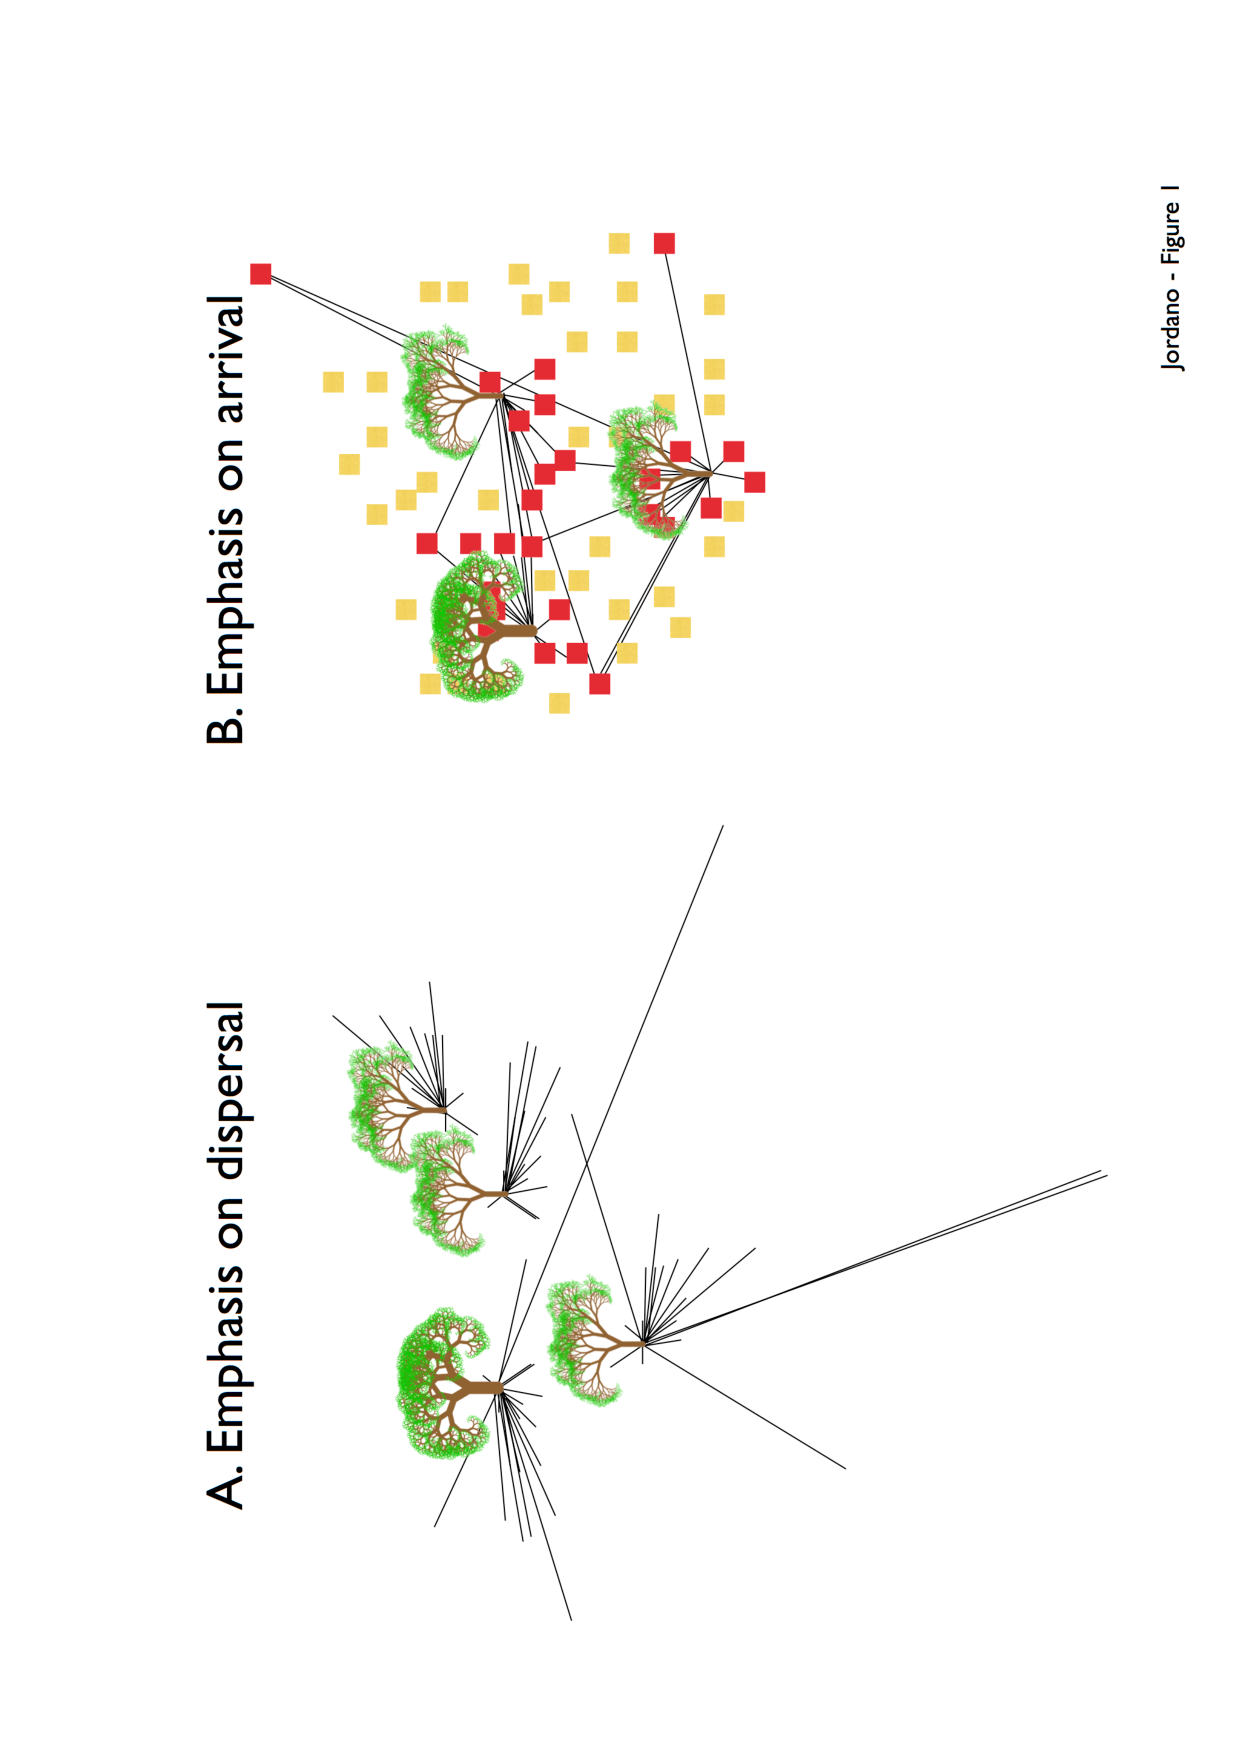
\includegraphics[height=25cm]{Fig1.pdf}}
%
%\caption{***}
\end{figure}

\newpage 
%------------------------------------------------------------------- Figure 2
\begin{figure}[htbp]
\centerline{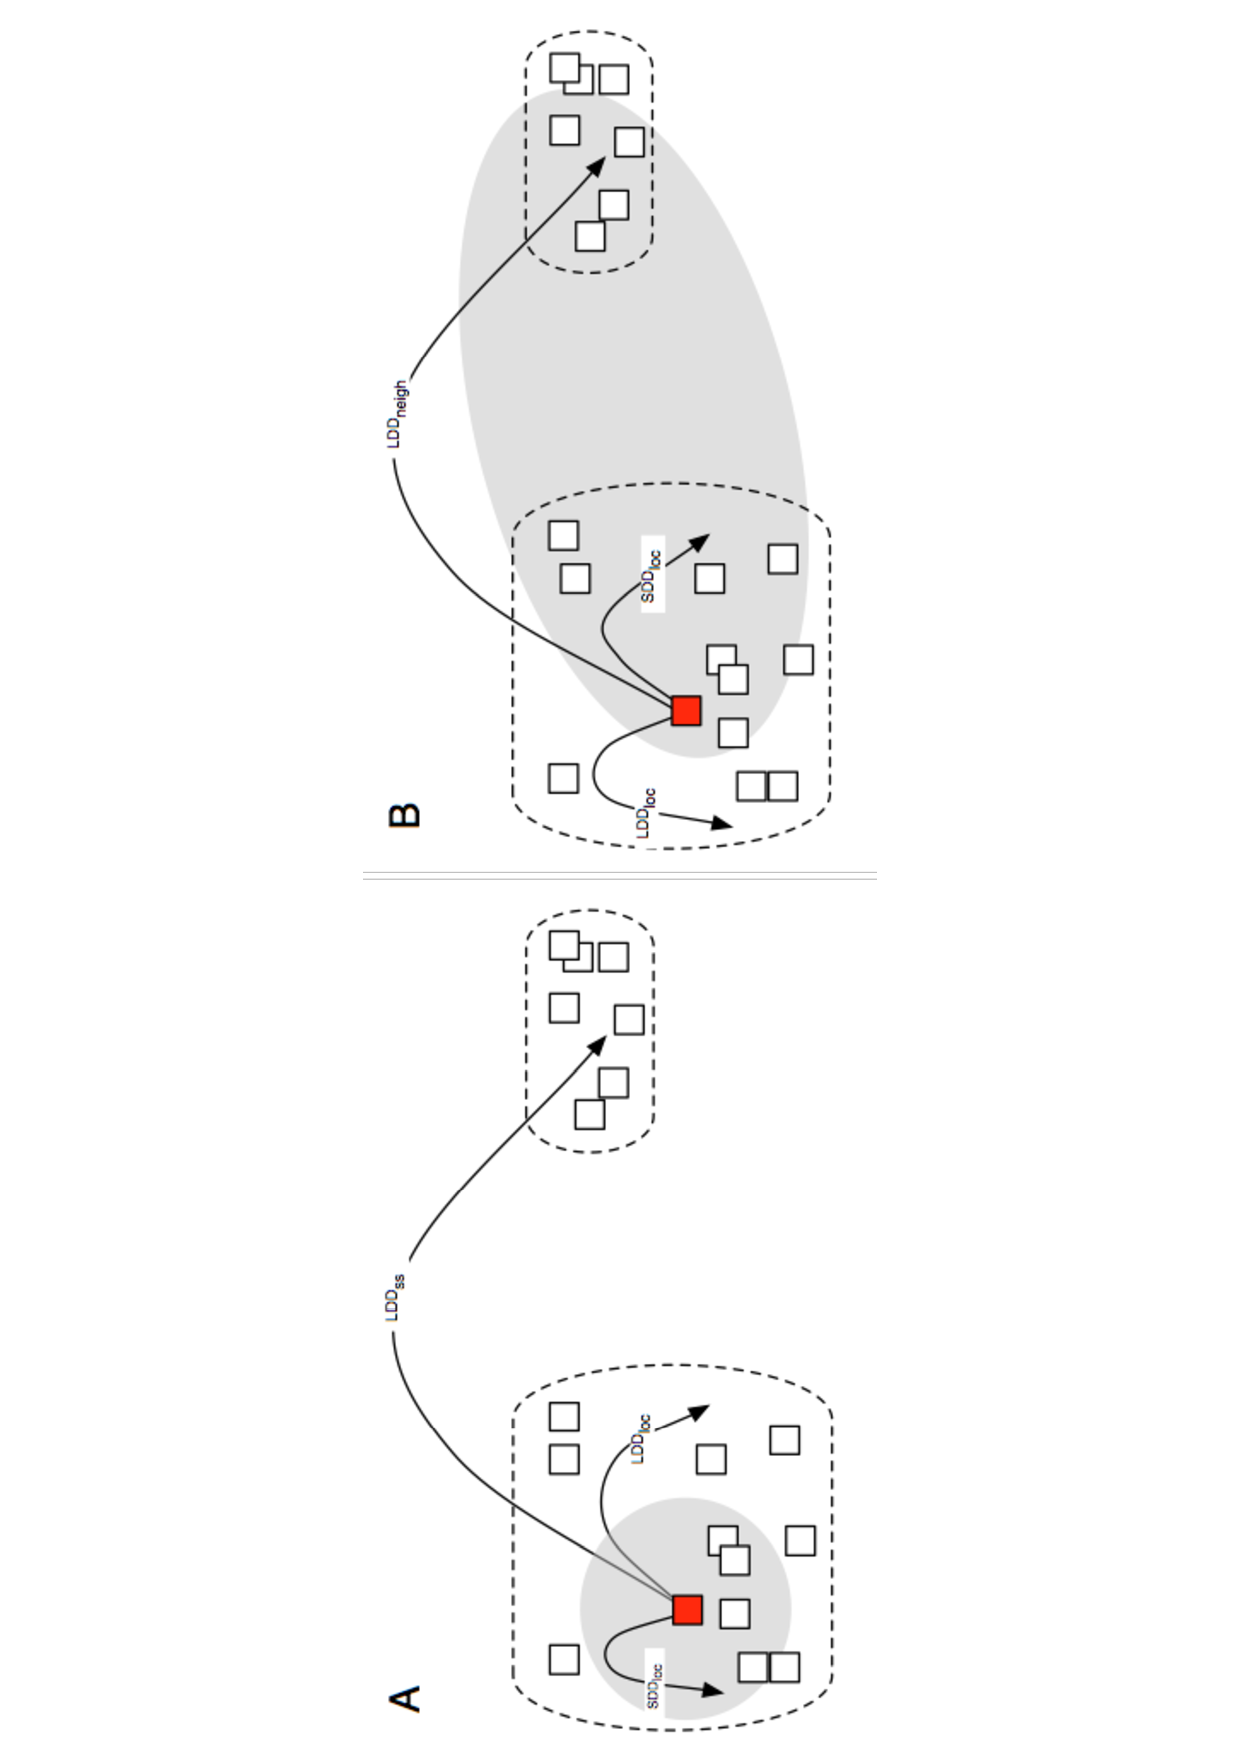
\includegraphics[height=25cm]{Fig2.pdf}}
%
%\caption{***}
\end{figure}

\newpage 
%------------------------------------------------------------------- Figure 3
\begin{figure}[htbp]
\centerline{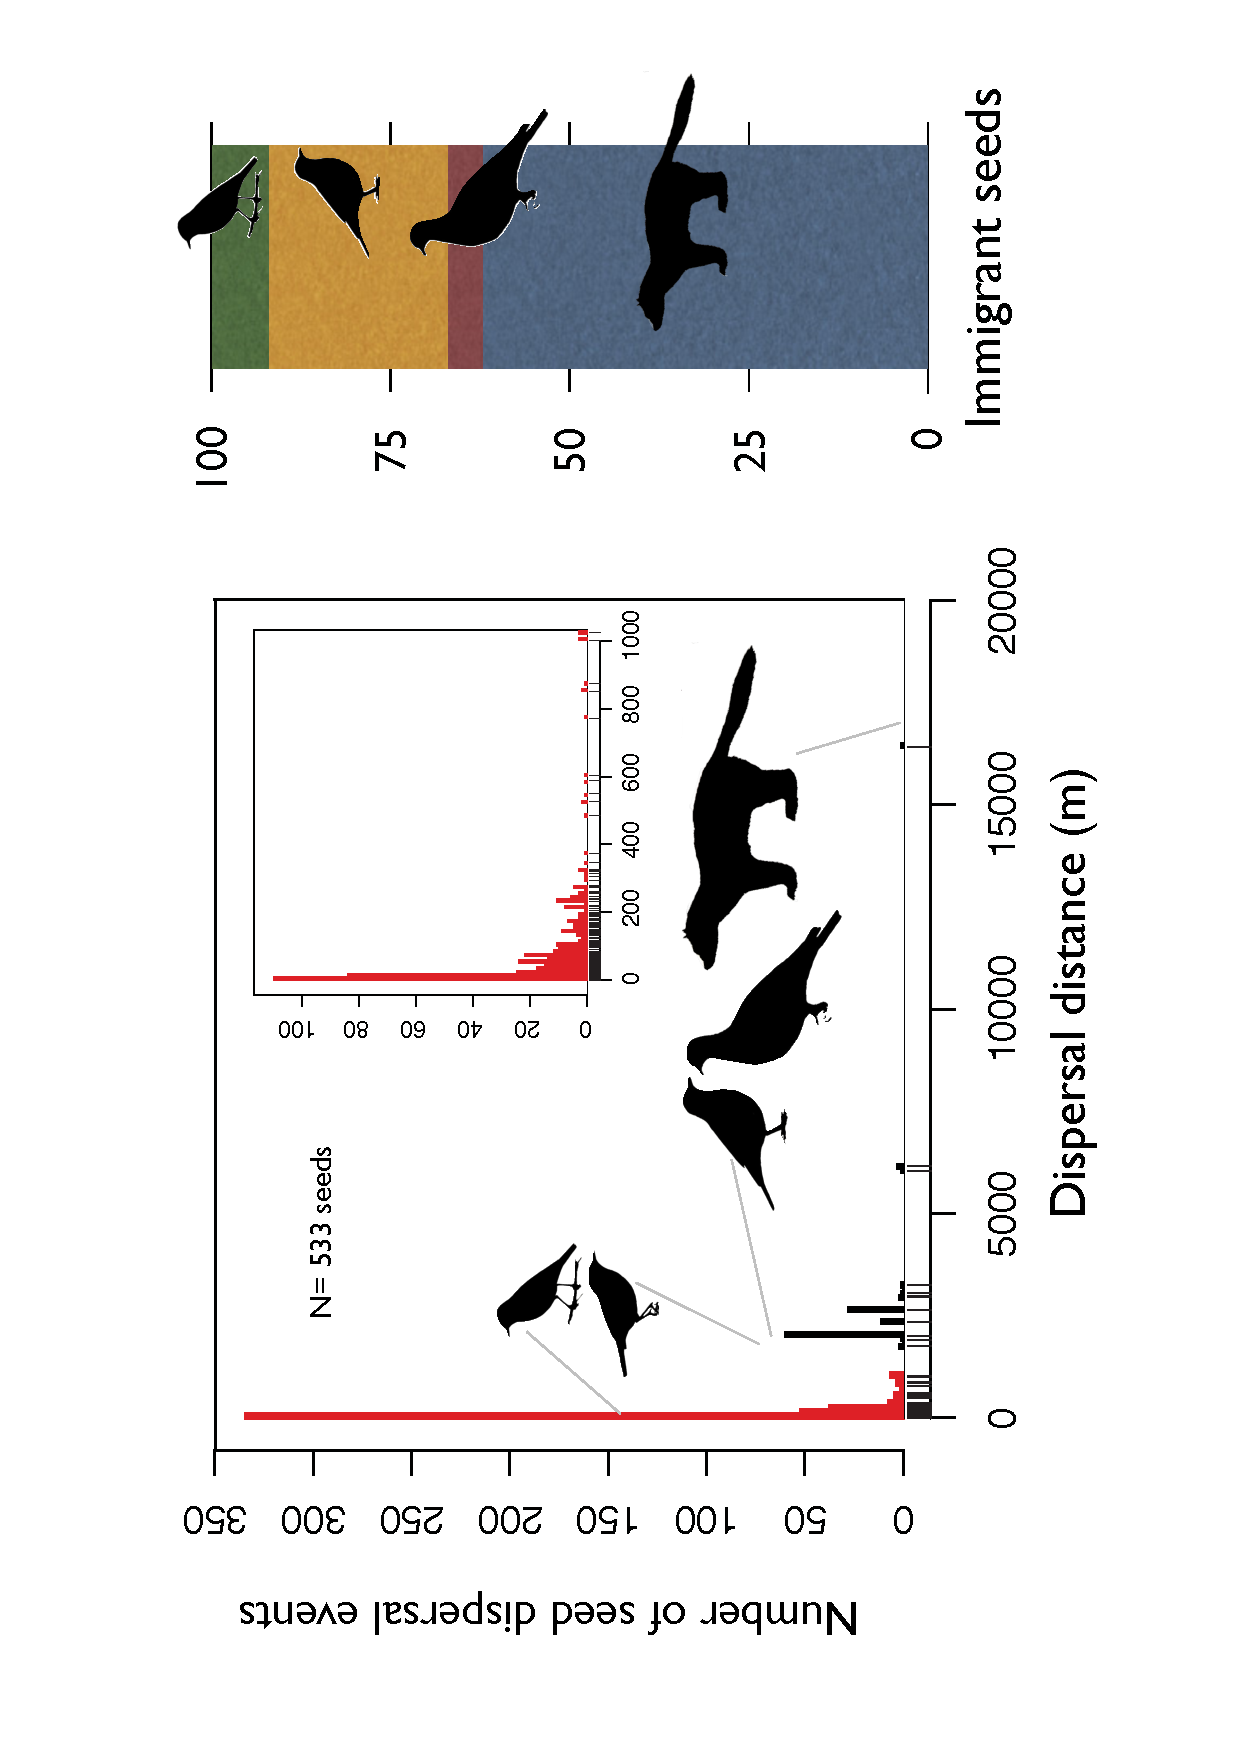
\includegraphics[height=26cm]{Fig3.pdf}}
%
%\caption{***}
\end{figure}
%----------------------------------------------------------------------------

\newpage 
%------------------------------------------------------------------- Figure 4
\begin{figure}[htbp]
\centerline{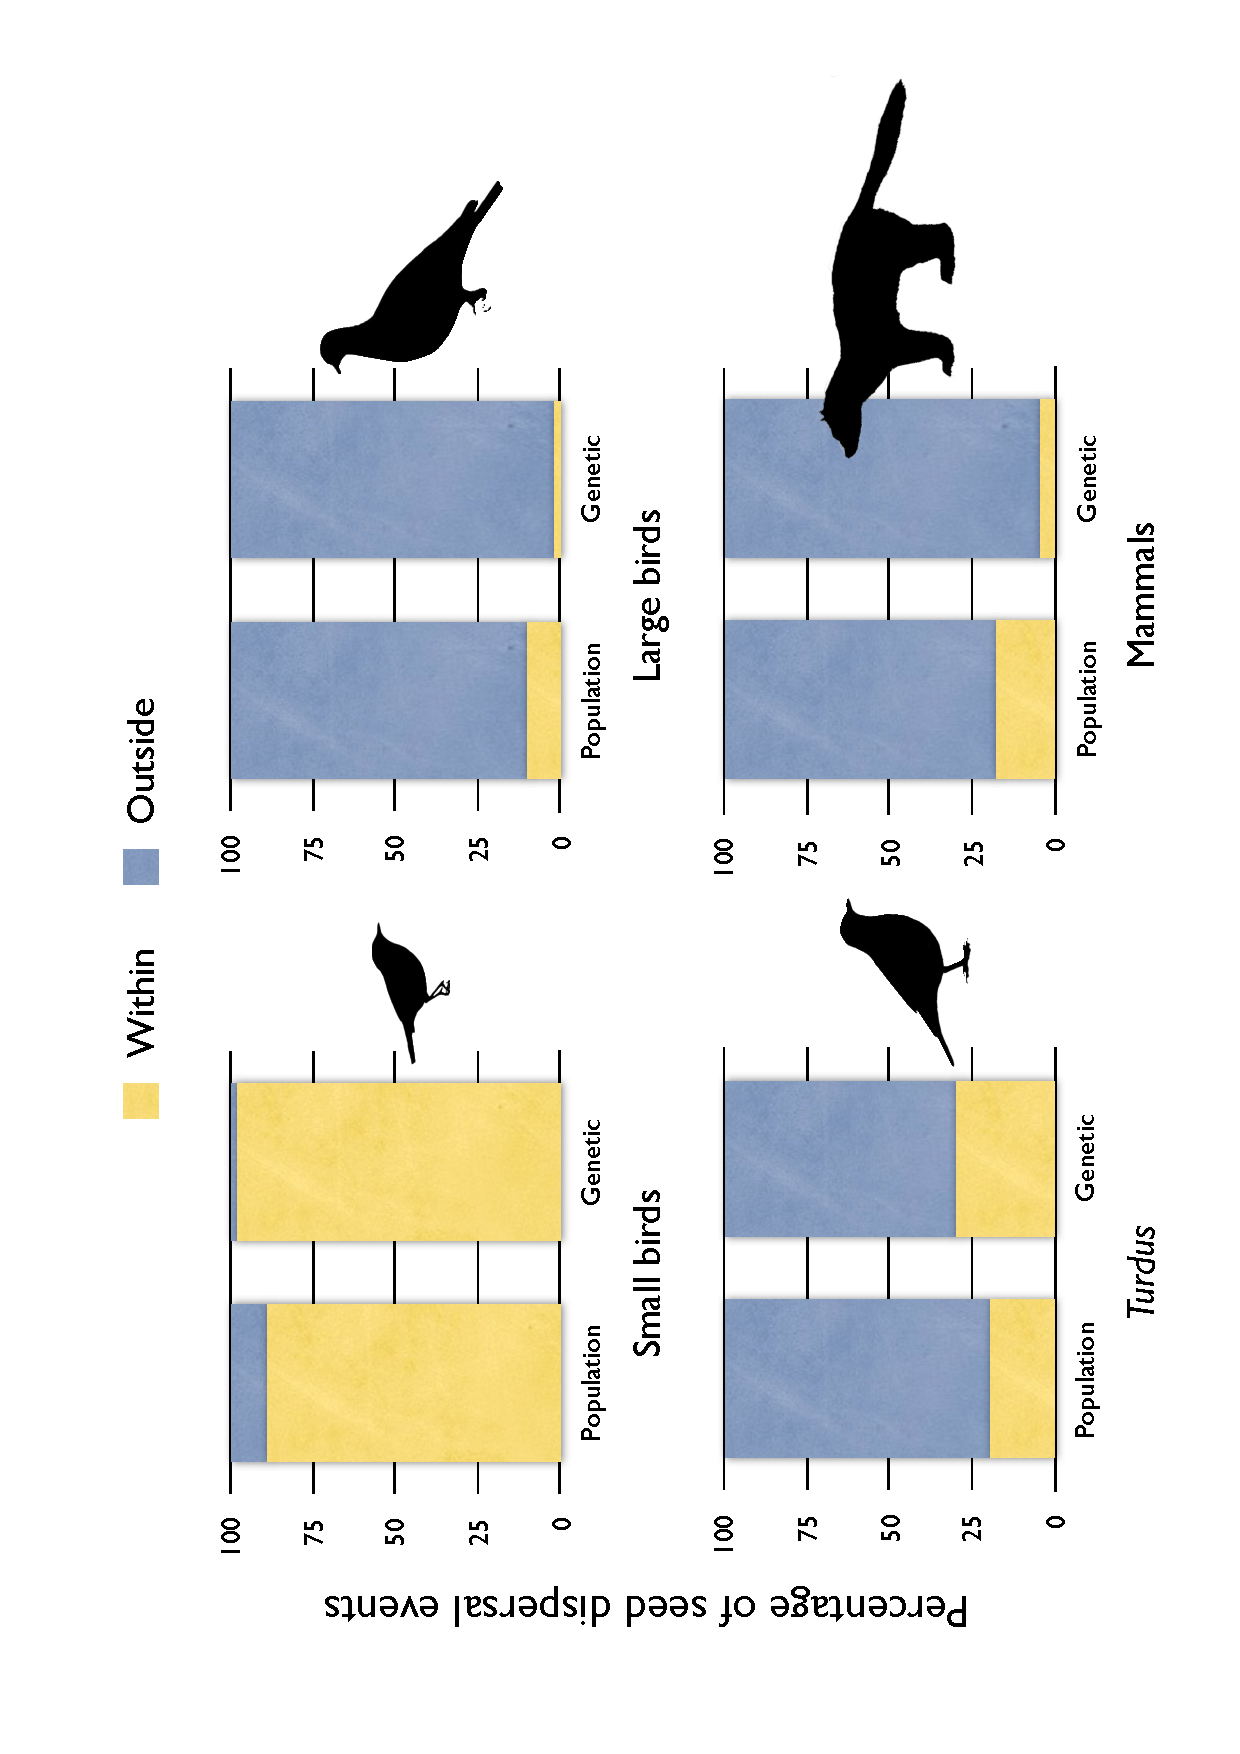
\includegraphics[height=25cm]{Fig4.pdf}}
%
%\caption{***}
\end{figure}

\newpage 

%%%%%%%%%%%%%%%%%%%%%%%%%%%%%%%%%%%%%%%%%%%%%%%%%%%%%%%%%%%%%%%%%%%%%%%%%%%%%%
\section*{Online Support Material and data accessiblity}

This review does not use new raw data, but includes some re-analyses of previously published material. All the original data supporting the paper, R code, supplementary figures, and summaries of analytical protocols is available at the author's GitHub repository (\texttt{https://github.com/pedroj/MS\_LDD}), with DOI: \texttt{\#/zenodo.\#}.
%%%%%%%%%%%%%%%%%%%%%%%%%%%%%%%%%%%%%%%%%%%%%%%%%%%%%%%%%%%%%%%%%%%%%%%%%%%%%%

\end{linenumbers}

%%%%%%%%%%%%%%%%%%%%%%%%%%%%%%%%%%%%%%%%%%%%%%%%%%%%%%%%%%%%%%%%%%%%% MS NOTES
\begin{comment}
NOTES
Breeding unit size. Donor number is related to the size of the breeding unit (N individuals) as d= Np, where d is the number of different pollen parent genotypes represented in a maternal tree’s fruit crop and p is the expected proportion of trees in staminate phase at any given time. Assuming, conservatively, that individual trees reproduce asynchronously twice per year 6 and that staminate and pistillate flowering phases each last seven days 20, p is calculated to be 0.0712. Although these estimates could be effected by mosaicism 21 (the fusion of genetically distinct individuals), its frequency in the species examined here is low. 

Breeding unit area and radii. These parameters were calculated from paternity-analysis-based estimates of breeding unit size (Nˆdˆ; Table2) and the censused densities of adult, reproductively mature trees over 15 km2 BCI. Based on the long-term censuses of C. Handley and E. Kalko, 6, 108 and 20 adults of F. dugandii, F. obtusifolia and F. popenoei, respectively, are known to occur on BCI. Because these species exhibit little spatial aggregation over the area censused, these densities are assumed to be representative of forested areas surrounding BCI, a conservative assumption given that approximately one-third of the area within 10 km of BCI is occupied by Lake Gatun where figs are absent. Breeding unit radii estimate the distances pollen-bearing, female fig wasps routinely disperse in search of receptive host trees. Although actual breeding populations of figs may deviate substantially from the assumed circular distribution, alternative structures (elliptical,for example)increase estimated wasp dispersal distances. 

\begin{itemize}
\item Levin’s paternity pool concept.  Levin, D. A. The paternity pools of plants. Am. Nat. 132, 309–317 (1988).
\end{itemize}

[Burnham, K.P. \& Overton, W.S. Robust estimation of population size when capture probabilities vary among animals. Ecology 60, 927–936 (1979).]

\paragraph*{Genetic ‘neighborhood’}

For continuously distributed populations, Wright (1946) introduced the concept of a genetic ‘neighborhood’ that describes the local area within which most matings occur. In a two-dimensional land- scape, Wright’s neighborhood size (NS) is  

\$NS = 4pisigma\textasciicircum{}2 D\$  

where D is density (number of individuals per unit area) and \$sigma\$ (mean squared distance along one axis between birthplaces of parents and their offspring) is a measure of dispersal. \emph{NS} can be thought of as the number of reproducing individuals in a circle of radius \$2sigma\$. Assuming that dispersal is Gaussian, a circle of this size would include \textasciitilde{}87 \% of the potential parents of individuals at the center (Wright, 1946).

If the dispersal of an individual between place of birth and breeding site is essentially random, it resembles a "drunkards walk". It has the same distribution as passive diffusion, a two-dimensional normal distribution.

If this is true, dispersal distance can simply measured as the standard deviation, \$sigma\$, of the dispersal distribution.  A population "neighbourhood" can be defined approximately as a group of individuals who come from an area \$2sigma\$ wide.

[Strictly, \$sigma\$ is a valid measure of dispersal only if dispersal is exactly normally distributed. Many field studies have shown that dispersal is actually leptokurtic, i.e. most offspring breed very close to their parents, but some breed an enormous distance away. In practice, it doesn't much matter if dispersal is non-normal, provided it is not too extreme.]

%%%%%%%%%%%
https://www.nceas.ucsb.edu/nceas-web/projects/2057/nceas-paper3/data/GFBoxB.html
%%%%%%%%%%%
Continuous populations can be modeled with the concepts of isolation by distance and neighborhood size\citep{Wright:1943aa,Wright:1946aa}. The former refers to the case that limited gene dispersal in continuous populations produces demes that are panmictic internally, but are isolated to some extent, from adjacent demes. Each group of reproducing individuals is the neighborhood, defined as the population of a region in a continuum, from which the parents of individuals born near the center may be treated as if drawn at random \citep{Wright:1969mb}. If distances between parents and offspring follow a normal distribution, the effective population size of the neighborhood will be:

$N_b= 4p \sigma^{2d}$

where $d$ is the density of adults per unit area and $\sigma$ is the variance in distance between birth and breeding sites. This is the basic model of ‘Isolation by Distance’ proposed by Wright  (1943, 1946). Under this type of model, migration (gene flow) is given by the variance in dispersal, and not by the proportion of the population that is composed of migrants (denoted $m$), as is the case with island models (Slatkin 1989).

For plants, gene flow may be accomplished by both seeds and pollen, so the variance may be decomposed to account for different patterns of seed and pollen dispersal, and to take into account the mating system (outcrossing rate, $t$). Thus, neighborhood size can be defined with the following equation (Crawford 1984) :

$N_b = 4p (\sigma^2_s + \frac{t \sigma^2_p}{2}) d (1 + t)$

where $\sigma^2_s$ is the variance in seed dispersal, $\sigma^2_s$ is the variance in pollen dispersal and $d$ is the density of potential parents.

Neighborhood size in plants can be estimated by marking pollen and seeds with fluorescent dyes, tags, or  marks. However, these methods do not measure effective pollen or seed movement, but they may be combined with genetic analysis to do so.  Individuals with a unique allele in a stand can provide valuable insight on seed movement \citep{Eguiarte:1993aa}.

\end{comment}
%%%%%%%%%%%%%%%%%%%%%%%%%%%%%%%%%%%%%%%%%%%%%%%%%%%%%%%%%%%%%%%%%%%%%%%%%%%%%

\end{document}
